\newpage
\section{Complex Attribute Manipulation}
\genHeader

\insertNoteAboutOptionalFeatures{Complex attribute manipulation}

Instead of going through the whole of this part, you may simply fetch the final state of the handbook example via \menuPath{Install Workspace \menuSep eMoflon Examples \menuSep Handbook Part 3 Final}.

In \Cref{sec: Implementing check} we have modeled the \texttt{Partition::check()} method.
However, as you might realized, our implementation ignores the \texttt{partitionSize}, \idest, the maximal number of cards that fit in a partition.
To prevent our implementation from \enquote{bursting} a partition we will use \emph{complex attribute constraints} to extend the SDM for the \texttt{Partition::check()} method. 
In contrast to simple attribute constrains\footnote{First used in \Cref{sec: Implementing check} to compare user’s guess against the card's face value}, which provide only binary operations for comparing attribute values (or literals), complex attribute constraints provides a language to specify arbitrary relations on attributes.

\subsection{Using Complex Attribute Constrains}     
We start by extending the \texttt{penalizeCard} pattern of the \texttt{Partition::check()} method in such a way that it only moves a card to the previous partition if the additional card does not exceed the actual \texttt{partitionSize} of the previous partition.
First, we extend \texttt{Partition} class by an attribute that keeps track of the actual number of card contained in a partition.
\begin{figure}[htbp]
\begin{center}
  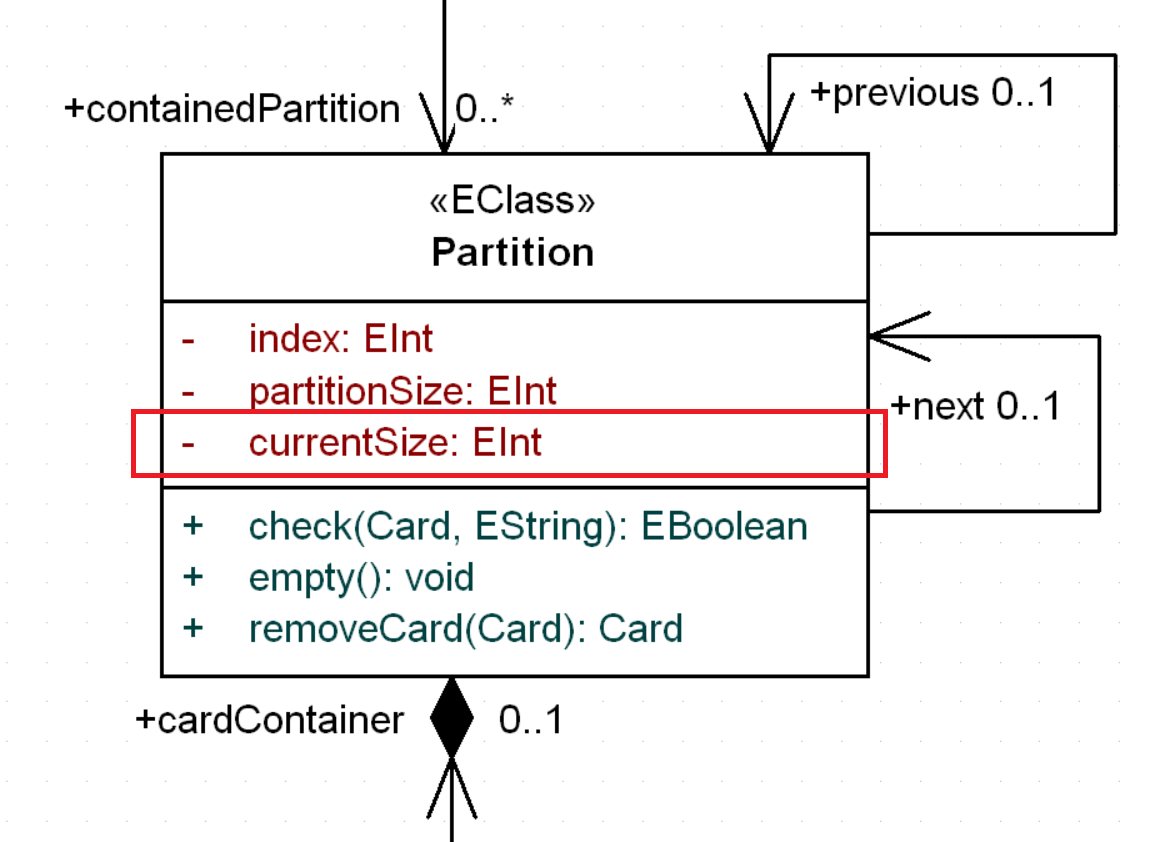
\includegraphics[width=0.4\textwidth]{ea_CAC_newAtributes}
  \caption{Adding the attribute \texttt{currentSize} of type \entity{EInt} to \texttt{Partition}}  
  \label{ea_CAC_newAtributes}
\end{center}
\end{figure}
%
\begin{stepbystep}    
\item Add to the class \texttt{Partition} the new attribute \texttt{currentSize:EInt} (\Cref{ea_CAC_newAtributes}).
\end{stepbystep} 
%
Now we start defining complex attribute constraints.
\begin{figure}[htbp]
\begin{center}
  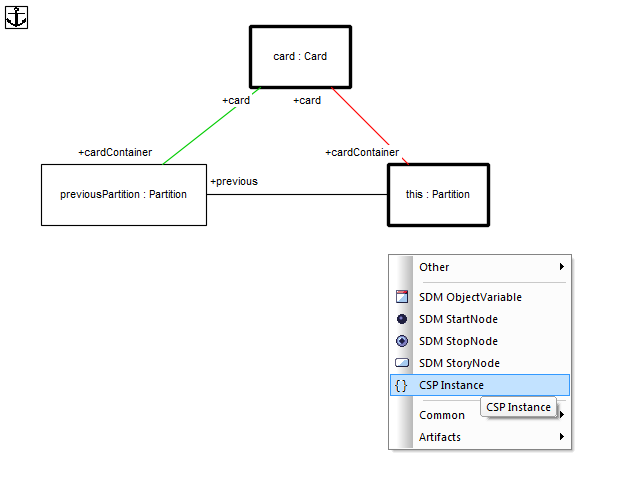
\includegraphics[width=0.8\textwidth]{ea_CAC_NewCSP}
  \caption{Creating a new \texttt{CSP instance}}  
  \label{ea:CAC_NewCSP}
\end{center}
\end{figure}
\begin{stepbystep}
%
\item Navigate to the \texttt{penalizeCard} pattern in the \texttt{Partition::check(Card,EString)} method and add a \texttt{CSP instance}.
Following a similar process as creating a new object variable, \idest, either hit space or use the toolbox to create a new \emph{CSP instance} (\Cref{ea:CAC_NewCSP}).
%
\item You’ll notice a box were you can specify your complex attribute constraints. Enter the attribute constraints as shown in \Cref{ea:ea_CAC_DefineCSP} to define that a card is only moved if the additional card does not exceed the actual \texttt{partitionSize} of the previous partition.

\end{stepbystep}

Before filling the text area with something meaningful, let's find out more about the general concepts of complex attribute constraints.
Basically, an attribute constraint is a predicate of the form

~~~~\texttt{SYMB(param$_1$,\ldots,param$_n$)}

\begin{itemize}
\item A \emph{predicate} \texttt{SYMB} specifies the relation of the affected parameters \texttt{param$_1$, \ldots, param$_n$}, \eg, equality \entity{=} or inequality \entity{!=}.
A parameter can be either a local variable, a constant or an attribute value, as defined in the following items.
    
\item A \emph{local variables} of the form \texttt{name:type}, \eg, \texttt{newCurrentSize : EInt} in \Cref{ea:ea_CAC_DefineCSP} defines an local variable \texttt{newCurrentSize} of type \texttt{EInt}. 

\item A \emph{constant} is of the form \texttt{value::type} (not the \emph{2} colons), \eg, \texttt{1::EInt} represents constant 1 of type \texttt{EInt}.

\item An \emph{attribute variable} is of the form \texttt{object\-Variable\-Name.attribute\-Name}, and refers to the current value of the attribute \texttt{attributeName} of object variable 	\texttt{object\-Variable\-Name}, while an attribute variable of the form \texttt{object\-Variable\-Name\-.attribte\-Name'} refers to an attribute value after the transformation.
This is necessary, \eg, to increment the attribute \entity{a} of variable \entity{x} as follows: \entity{+(x.a', x.a, 1::EInt)}. 

\item A \emph{package import} is of the form \entity{importPackage packageName;} and specifies that the package \entity{packageName} should be used to search for types.
For instance, \entity{importPackage Ecore;} is required to refer to the type \entity{EInt}. 
\end{itemize}
%
Enough theory for now:
Let's get back to the example.
\begin{stepbystep}
\item Insert the following lines (\texttt{importPackage Ecore;} should be already there) to reflect \Cref{ea:ea_CAC_DefineCSP}.
Especially, make sure that the \menuPath{NAC index} is set to \entity{-1}.
Double-slashes may be used to add single-line comments.
\begin{verbatim}
// Required to use (e.g.,) datatype EInt
importPackage Ecore;

// Introduces a temporary variable to store the (tentative) new
// size of the previous partition
+(newCurrentSize:EInt, previousPartition.currentSize, 1::EInt);

// Check that the tentative size does not exceed the capacity
// of the previous partition.
<=(newCurrentSize:EInt, previousPartition.partitionSize);

// Decrement size of current partition
-(this.currentSize', this.currentSize, 1::EInt);

// Increment size of previous partition
=(previousPartition.currentSize', newCurrentSize:EInt);
\end{verbatim}
%
\begin{figure}[htbp]
    \begin{center}
        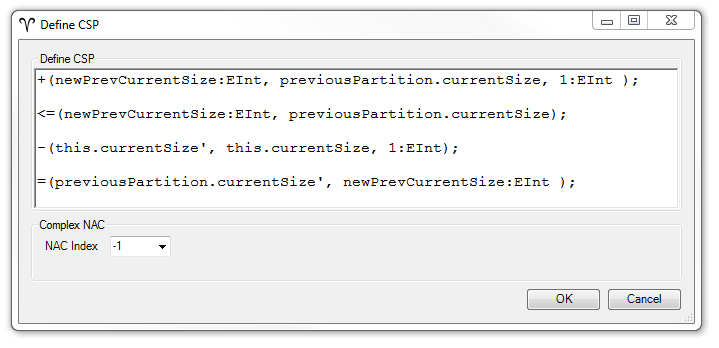
\includegraphics[width=0.9\textwidth]{ea_CAC_DefineCSP}
        \caption{Attribute constraints that prevent exceeding the partition size}  
        \label{ea:ea_CAC_DefineCSP}
    \end{center}
\end{figure}
% 
\item
Export the project as usual. 
Before generating code, you have to switch the code generation engine.
Open \entity{moflon.properties.xmi} located in your project and change the \menuPath{SDM Codegenerator Method Body Handler} to  \entity{DEMOCLES\_ATTRIBUTES} (\Cref{ec_CAC_SwitchCGE}).

\begin{figure}[htbp]
\begin{center}
  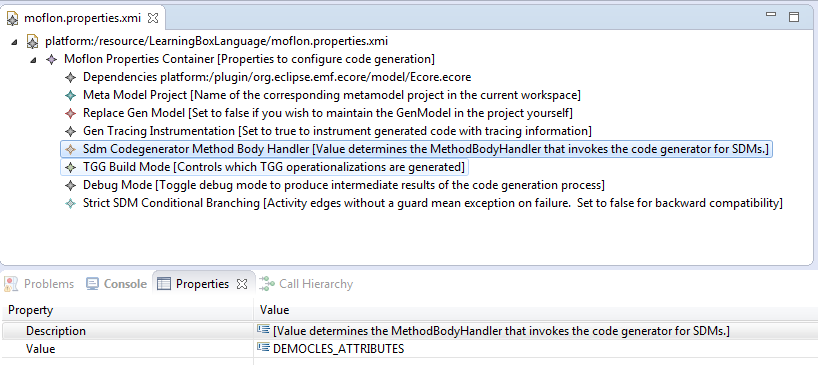
\includegraphics[width=0.99\textwidth]{ec_CAC_SwitchCGE}
  \caption{Switching SDM code generator to \entity{DEMOCLES\_ATTRIBUTES}}  
  \label{ec_CAC_SwitchCGE}
\end{center}
\end{figure}

\end{stepbystep}
The code generator engine is now able to solve the CSP instances, \idest, the constraints are operationalized and put in correct order. 
The code resulting for the CSP instance is shown in \Cref{ea_CAC_penalizeCardLHS,ea_CAC_penalizeCardRHS} for the LHS and RHS, respectively.
\begin{figure}[htbp]
\begin{lstlisting}[language=Java, keywordstyle={\bfseries\color{purple}}]
int this_currentSize = _this.getCurrentSize();

int previousPartition_currentSize = 
  previousPartition.getCurrentSize();
  
int previousPartition_partitionSize = 
  previousPartition.getPartitionSize();
  
int this_currentSize_prime = this_currentSize - 1;

int newCurrentSize = previousPartition_currentSize + 1;

if (newCurrentSize <= previousPartition_partitionSize) {
    int  previousPartition_currentSize_prime = newCurrentSize;
    // return match
}
\end{lstlisting}
\caption{LHS pattern code generated for the CSP instance}
\label{ea_CAC_penalizeCardLHS}
\end{figure}
    

\begin{figure}[htbp]
\begin{center}
\begin{lstlisting}[language=Java, keywordstyle={\bfseries\color{purple}}]
_this.setCurrentSize(Integer.valueOf(this_currentSize_prime));

previousPartition.setCurrentSize(
  Integer.valueOf(previousPartition_currentSize_prime));
\end{lstlisting}
\caption{RHS pattern code generated for the CSP instance}  
\label{ea_CAC_penalizeCardRHS}
\end{center}
\end{figure}

Notice that the attribute variables \texttt{this.currentSize'} and \\
\texttt{previousPartition.currentSize'} (represented in the code by \\ 
\texttt{this\_currentSize\_prime} and \texttt{previousPartition\_currentSize\_prime}, respectively) are treated as local variables on the LHS and then assigned on the RHS to the corresponding attribute values.
%Hence, we might rewrite the \texttt{CSP instance} shown in \Cref{ea:ea_CAC_DefineCSP} to the more compact shown in \Cref{ea:ea_CAC_DefineCSP2}.
%\begin{figure}[htbp]
%\begin{center}
%  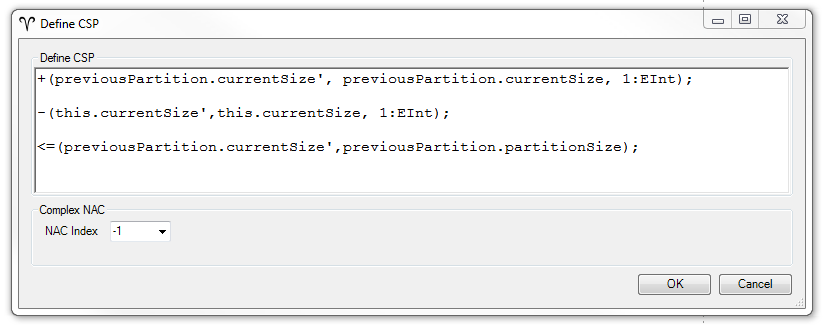
\includegraphics[width=0.99\textwidth]{ea_CAC_DefineCSP2}
%  \caption{Defining complex attribute constraints}  
%  \label{ea:ea_CAC_DefineCSP2}
%\end{center}
%\end{figure}

\subsection{Defining Your Own Complex Attribute Constraints}  
In \Cref{sec_A string representation of our learning box} we have implemented the \texttt{Box::toString()} method to obtain a string representation of the box. 
Internally, this method uses the method \texttt{Box::addToStringRep(Card) : EString} to create a string from a card, that was realized using handwritten code via injections.

In the following, we replace the method \texttt{Box::addToStringRep(Card):EString} by a complex attribute constraint.

\begin{stepbystep}
\item 
Reconsider the SDM shown in \Cref{ea:sdm_tostringComplete}.
First, add an attribute constraint for appending the string \texttt{"Content: "} to the \entity{stringRep} attribute of \entity{ Box}.
To this end, add to the \entity{ForAllPartitons} pattern the following complex attribute constraint:
\begin{verbatim}
+(this.stringRep', this.stringRep, "Content: "::EString)
\end{verbatim}
\end{stepbystep}  
Note that the predicate \entity{+} is overloaded: For \entity{EInt}, \entity{+} means integer addition, while for \entity{EInt}, it means concatenation.
   	  


In a next step, the pattern \entity{ForAllCards} is extended by an complex attribute constraints such that for each card the string containing the front and back is appended to \emph{this.stringRep}.  	 
Instead of using the the concatenation predicate \texttt{+} again, we just define our own constraint as follows.
\begin{stepbystep}
\item 
Add a \texttt{CSP instance} with the following content to the \texttt{ForAllCards} pattern.
\begin{verbatim}
myConcat(this.stringRep', this.stringRep, card.face, card.back);
\end{verbatim}
The complete SDM should now look as shown in \Cref{ea_CAC_CompletToString}.
%
\begin{figure}[htbp]
\begin{center}
  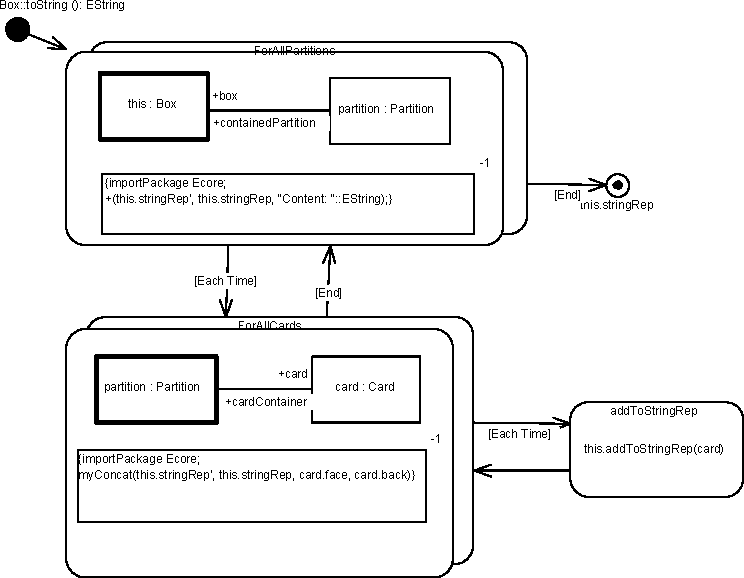
\includegraphics[width=0.99\textwidth]{ea_CAC_CompletToString.pdf}
  \caption{Complete SDM for \texttt{Box::toString()}}  
  \label{ea_CAC_CompletToString}
\end{center}
\end{figure}
%
Note that \entity{importPackage Ecore;} can be omitted in the constraints of \entity{ForAllCards} because no (Ecore) data types are used there.
%
\item
Export as usual.
If you are now building the metamodel project in Eclipse, you get an error message (\Cref{ec_CAC_Malformed}) that informs you that the attribute constraint with signature \\
\hspace*{0.5cm} \texttt{\small myConcat( :EString, :EString, :EString, :EString)} \\
is unknown.

\item
Look inside \texttt{LearningBoxLanguage/lib/}.
You find a new file called \texttt{LearningBoxLanguageAttributeConstraintsLib.xmi} 
 
\begin{figure}[htbp]
\begin{center}
  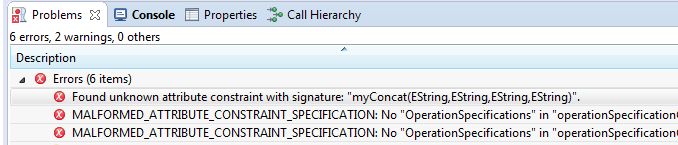
\includegraphics[width=0.99\textwidth]{ec_CAC_Malformed}
  \caption{Error}  
  \label{ec_CAC_Malformed}
\end{center}
\end{figure}



\item
Open the file.
It contains a constraint specification \texttt{myConcat} (\Cref{ec_CAC_lib} bottom) that represents the signature (\texttt{\small myConcat( :EString, :EString, :EString, :EString)}), which is derived from the information of the CSP-instance in EA.
To define the meaning of \texttt{myConcat} we have to define operations for the constraint.

\begin{figure}[htbp]
\begin{center}
  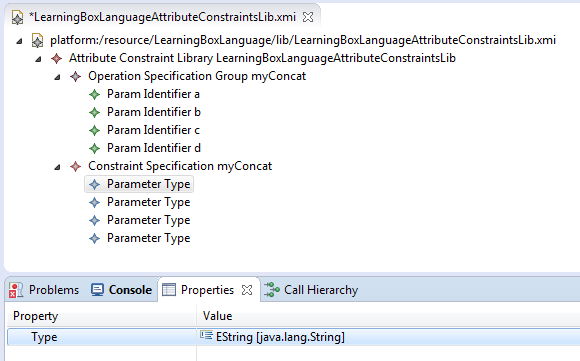
\includegraphics[width=0.95\textwidth]{ec_CAC_lib}
  \caption{\entity{LearningBoxLanguageAttributeConstraintsLib.xmi}}  
  \label{ec_CAC_lib}
\end{center}
\end{figure}
\item
Right click the operation specification group for \texttt{myConcat} (top of \Cref{ec_CAC_lib}) and add (as a new child) an \texttt{operation specification}. 
\end{stepbystep}

An operation\footnote{Double click on the operation specification to open the properties view.} is specified by an \emph{Adornment String}, and a \texttt{Specification} that is a template defining the code to be generated.

\begin{figure}[htbp]
\begin{center}
  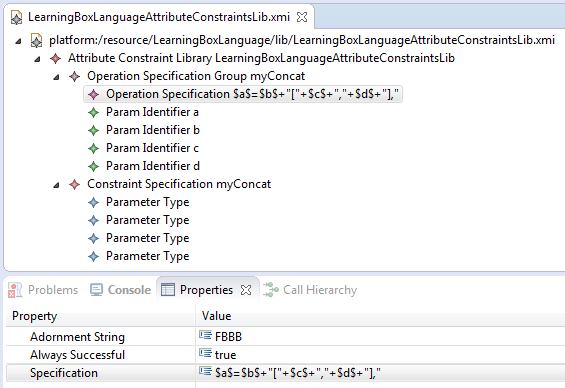
\includegraphics[width=0.99\textwidth]{ea_CAC_opSpec}
  \caption{Operation specification for \entity{myConcat}}  
  \label{ea_CAC_opSpec}
\end{center}
\end{figure}

\begin{itemize}
\item[$\blacktriangleright$] Complete the operation specification as shown in \Cref{ea_CAC_opSpec}. The adornment string \texttt{FBBB} means that before the operation can be executed the values for parameter \entity{b}, \entity{c}, and \entity{d} must be known (\idest, they are \texttt{b}ound), and that parameter \entity{a} is unknown (\idest, it is a \texttt{f}ree parameter).
Therefore, in the \entity{Specification} template, we add a formula that describes how \entity{a} can be derived based on \entity{b}, \entity{c}, and \entity{d}.
Inside the template code, the variables are refered to using \entity{\$}.
The surrounding code has to be valid Java code.
\end{itemize}

\subsection{Built-in Attribute Constraint Types}
%Please visit the following URL to get a full overview of supported attribute constraint types:\\
%{\footnotesize
%\url{https://github.com/eMoflon/emoflon/wiki/Attribute-Constraints-Library}}.  
\begin{longtable}{clr} \toprule
\textbf{Symbol} & \textbf{Signatures}  & \textbf{Semantics}\\ \midrule 
\endhead
$=$ & (a:Eint , b:EInt) & $(a:=b)$ for \entity{FB} \\ 
 & (a:EDouble , b:EDouble) & $(a==b)$ for \entity{BB}\\ 
 & (a:EFloat , b:EFloat) &  \\ 
 & (a:EShort , b:EShort) & \\ 
 & (a:ELong , b:ELong) &  \\ 
 & (a:EString , b:EString) & \\\midrule
 $<=$ & (a:Eint , b:EInt) & $(a\leq b)$ for \entity{BB} \\ 
 & (a:EDouble , b:EDouble) & \\ 
 & (a:EFloat , b:EFloat) &  \\ 
 & (a:EShort , b:EShort) & \\ 
 & (a:ELong , b:ELong) &  \\\midrule
 $<$ & (a:Eint , b:EInt) & $(a < b)$ for \entity{BB}\\ 
 & (a:EDouble , b:EDouble) & \\ 
 & (a:EFloat , b:EFloat) &  \\ 
 & (a:EShort , b:EShort) & \\ 
 & (a:ELong , b:ELong) &  \\\midrule
 $>=$ & (a:Eint , b:EInt) & $(a\geq b)$ for \entity{BB}\\ 
 & (a:EDouble , b:EDouble) & \\ 
 & (a:EFloat , b:EFloat) &  \\ 
 & (a:EShort , b:EShort) & \\ 
 & (a:ELong , b:ELong) &  \\\midrule
 $>$ & (a:Eint , b:EInt) & $(a > b)$ \entity{BB}\\ 
 & (a:EDouble , b:EDouble) & \\ 
 & (a:EFloat , b:EFloat) &  \\ 
 & (a:EShort , b:EShort) & \\ 
 & (a:ELong , b:ELong) &  \\\midrule
$+$ & (a:Eint , b:EInt, c:EInt) & $(a=b+c)$ for \entity{FBB} \\ 
 & (a:EDouble, b:EDouble,c:EDouble) & \\ 
 & (a:EFloat , b:EFloat, c:EFloat) &  \\ 
 & (a:EShort , b:EShort, c:EShort) & \\ 
 & (a:ELong , b:ELong, c:ELong) &  \\ 
 & (a:EString , b:EString, c:EString) & \\\midrule
$-$ & (a:Eint , b:EInt, c:EInt) & $(a=b-c)$ for \entity{FBB}\\ 
 & (a:EDouble,b:EDouble,c:EDouble) & \\ 
 & (a:EFloat , b:EFloat, c:EFloat) &  \\ 
 & (a:EShort , b:EShort, c:EShort) & \\ 
 & (a:ELong , b:ELong, c:ELong) &  \\ \midrule
$ /$ & (a:Eint , b:EInt, c:EInt) & $(a=b/c)$ for \entity{FBB}\\ 
 & (a:EDouble,b:EDouble,c:EDouble) & \\ 
 & (a:EFloat , b:EFloat, c:EFloat) &  \\ 
 & (a:EShort , b:EShort, c:EShort) & \\ 
 & (a:ELong , b:ELong, c:ELong) &  \\ \midrule
$ *$ & (a:Eint , b:EInt, c:EInt) & $(a=b\cdot c)$ for \entity{FBB}\\ 
 & (a:EDouble,b:EDouble,c:EDouble) & \\ 
 & (a:EFloat , b:EFloat, c:EFloat) &  \\ 
 & (a:EShort , b:EShort, c:EShort) & \\ 
 & (a:ELong , b:ELong, c:ELong) &  \\ \bottomrule
  \end{longtable}





   
